\documentclass[xetex,mathserif,serif]{beamer}
\usepackage{polyglossia}
\setdefaultlanguage[babelshorthands=true]{russian}
\usepackage{minted}

\useoutertheme{infolines}

\setmainfont{FreeSans}
\newfontfamily{\russianfonttt}{FreeSans}

\definecolor{links}{HTML}{2A1B81}
\hypersetup{colorlinks,linkcolor=,urlcolor=links}

\title{Учебные практики на кафедре СП}
\subtitle{Требования, рекомендации}
\author[Юрий Литвинов]{Юрий Литвинов \newline \textcolor{gray}{\small\texttt{yurii.litvinov@gmail.com}}}
\date{08.12.2020г}

\begin{document}
    
    \frame{\titlepage}

    \begin{frame}
        \frametitle{Что такое учебная практика}
        \begin{itemize}
            \item Научно-исследовательская или программно-инженерная работа
            \begin{itemize}
                \item Решение более-менее научной или практически полезной задачи
                \item Отчёт (текст)
                \item Код (опционально, но желательно)
            \end{itemize}
            \item По формату близка к научной статье и выступлению на конференции
            \item Тема должна быть интересна кафедре (``программирование для программистов'')
        \end{itemize}
    \end{frame}

    \begin{frame}
        \frametitle{Требования}
        \begin{itemize}
            \item Отчёт
            \begin{itemize}
                \item Порядка 10 страниц
                \item К 15 декабря
                \item Выборочное рецензирование
            \end{itemize}
            \item Доклад
            \begin{itemize}
                \item Порядка 3-5 минут
                \item Рассказать о задаче и текущих успехах
            \end{itemize}
            \item Отзывы научного руководителя и консультанта
            \item Ссылка на код, если он открыт
        \end{itemize}
    \end{frame}

    \begin{frame}
        \frametitle{Полезные ресурсы}
        \begin{itemize}
            \item Рассылка кафедры --- \url{http://bit.ly/sysprog-talks}
            \item Рассылка курса --- \url{https://groups.google.com/g/spbsu-se-bachelors-2018-2022}
            \item Команда Teams курса --- \textbf{fuhddmr}
            \begin{itemize}
                \item Подписаться обязательно
            \end{itemize}
            \item Сайт кафедры --- \url{http://oops.math.spbu.ru/SE}
            \begin{itemize}
                \item Раздел ``Студенту'' --- рекомендации, архив работ
            \end{itemize}
            \item Титульники --- по образу и подобию учебных практик 2-го курса
            \item Онлайн-редакторы TeX --- \url{https://papeeria.com/}, \url{https://www.overleaf.com/}
            \item Чеклист по презентациям --- \url{https://goo.gl/UeDRff}
        \end{itemize}
    \end{frame}

    \begin{frame}
        \frametitle{Отчёт, структура}
        \begin{itemize}
            \item Титульный лист
            \item Оглавление
            \item Введение в предметную область, постановка задачи
            \item Обзор литературы и существующих решений
            \item Описание предлагаемого решения (архитектура, план реализации, что успели сделать)
            \item Заключение
            \item Список литературы
        \end{itemize}
    \end{frame}

    \begin{frame}
        \frametitle{Оглавление}
        \begin{itemize}
            \item Все разделы, даже список литературы
            \item Точно повторять название глав текста
            \item Титульный лист не нумеруется
        \end{itemize}
    \end{frame}

    \begin{frame}
        \frametitle{Введение}
        \begin{columns}
            \begin{column}{0.6\textwidth}
                \begin{itemize}
                    \item Известная информация, ``Background''
                    \item Неизвестная информация, ``Gap''
                    \begin{itemize}
                        \item Актуальность темы
                        \item Практическая значимость
                        \item Кому конкретно это надо
                    \end{itemize}
                    \item Кратко про ваш подход к решению задачи, почему он приведёт к успеху (``Гипотеза'' и ``Подход'')
                \end{itemize}
            \end{column}
            \begin{column}{0.4\textwidth}
                \begin{center}
                    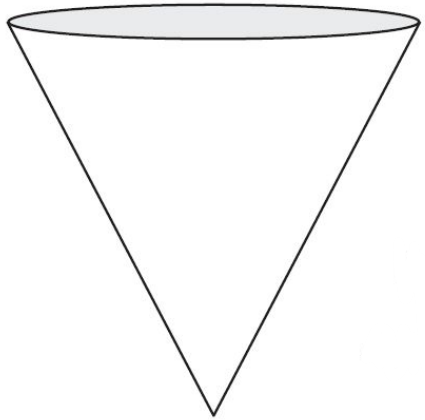
\includegraphics[width=\textwidth]{introductionCone.png}
                \end{center}
            \end{column}
        \end{columns}
    \end{frame}

    \begin{frame}
        \frametitle{Постановка задачи}
        \begin{itemize}
            \item Цель работы
            \begin{itemize}
                \item Одним предложением --- что конкретно надо сделать
            \end{itemize}
            \item Задачи
            \begin{itemize}
                \item Отчуждаемые
                \item Специфичные
                \item Решение которых приведёт к цели
                \item Выполнить обзор, спроектировать, реализовать, выполнить апробацию/эксперименты
                \item Отдельно на осеннюю и весеннюю часть
            \end{itemize}
        \end{itemize}
    \end{frame}

    \begin{frame}
        \frametitle{Обзор}
        \begin{itemize}
            \item Обзор существующих решений
            \begin{itemize}
                \item Цель обзора, критерии отбора материалов
                \item Критерии сравнения
                \item Таблица с результатами
                \item Выводы
            \end{itemize}
            \item Обзор используемых чужих результатов
            \begin{itemize}
                \item  Всё, написанное и придуманное не вами --- в обзор
            \end{itemize}
            \item Должен соотноситься с темой работы
        \end{itemize}
    \end{frame}

    \begin{frame}
        \frametitle{Описание решения}
        \begin{itemize}
            \item Потом будет несколько разделов, сейчас достаточно одного
            \begin{itemize}
                \item Желательно, чтобы разделы соответствовали списку задач
            \end{itemize}
            \item Аргументированное обоснование принятых решений и отказа от альтернатив
            \item Выбор инструментария
            \item Описание архитектуры, алгоритмов и т.п.
        \end{itemize}
    \end{frame}

    \begin{frame}
        \frametitle{Описание решения (2)}
        \begin{itemize}
            \item Рисунки и диаграммы
            \begin{itemize}
                \item Лучше использовать UML --- он стандартный
                \item Подписи
                \begin{itemize}
                    \item Чужие рисунки --- со ссылкой на источник
                \end{itemize}
                \item Ссылки из текста
                \item Сквозная нумерация
            \end{itemize}
            \item Таблицы
            \begin{itemize}
                \item Чтобы было всё видно даже в напечатанном варианте
            \end{itemize}
        \end{itemize}
    \end{frame}

    \begin{frame}
        \frametitle{Заключение}
        \begin{itemize}
            \item Перечисление результатов, выносимых на защиту сейчас
            \item Должно быть согласовано с постановкой задачи (вплоть до полного её повторения)
            \item Должно быть согласовано с текстом
            \begin{itemize}
                \item Никаких результатов из ниоткуда
            \end{itemize}
            \item Реалистичные планы на весну
            \item Примерно полстраницы
        \end{itemize}
    \end{frame}

    \begin{frame}
        \frametitle{Литература}
        \begin{itemize}
            \item Cсылок примерно как страниц в работе
            \item Обязательно на каждый пункт ссылаться из текста
            \item Лучше ссылаться на научные статьи
            \begin{itemize}
                \item Ещё лучше --- на книги, но по предметной области
                \item Смотрите на индекс Хирша и число цитирований
            \end{itemize}
            \item Реально прочитанные работы
            \begin{itemize}
                \item Всё-таки прочитать бывает полезно
            \end{itemize}
        \end{itemize}
    \end{frame}

    \begin{frame}
        \frametitle{Литература (2)}
        \begin{itemize}
            \item ГОСТ Р 7.0.5-2008
            \begin{itemize}
                \item А.Н. Терехов, Т.А. Брыксин, Ю.В. Литвинов и др., Архитектура среды визуального моделирования QReal. // Системное программирование. Вып. 4. СПб.: Изд-во СПбГУ. 2009, С. 171-196
                \item Порядок --- алфавитный (по авторам), в порядке упоминания в тексте, в хронологическом порядке (если это важно)
                \item Ссылки в тексте --- номер в квадратных скобках: ``блаблабла [1]'' (с пробелом)
            \end{itemize}
            \item В литературу --- только, гм, литературу
            \begin{itemize}
                \item Подстраничные сноски для ссылок на сайты, статьи на Хабре и т.д.
                \item Электронные источники в списке литературы допустимы (надо указывать дату обращения)
            \end{itemize}
        \end{itemize}
    \end{frame}

    \begin{frame}
        \frametitle{Презентация, структура}
        \begin{itemize}
            \item Титульный слайд
            \item Введение (примерно 1-2 слайда)
            \item Постановка задачи (1 слайд)
            \item Обзор (примерно 1 слайд)
            \item Предлагаемое решение (примерно 1 слайд)
            \item Результаты, выносимые на защиту (1 слайд) --- обязательно, последним слайдом
        \end{itemize}
    \end{frame}

    \begin{frame}
        \frametitle{Общие рекомендации}
        \begin{itemize}
            \item Никакого заимствования 
            \begin{itemize}
                \item Сдача чужой работы --- отчисление без права восстановления сразу
                \item Копипаст даже одного предложения без указания источника --- незачёт
                \item Правильно оформленный копипаст --- попросят убрать
            \end{itemize}
            \item Обязательно показать и текст, и презентацию научнику
            \begin{itemize}
                \item Стоит порепетировать выступление
            \end{itemize}
            \item Из презентации должно быть предельно понятно, что и зачем вы делаете (актуальность, сложность работы) и при чём тут СП
            \begin{itemize}
                \item Будут яростно нападать
            \end{itemize}
            \item Озаботьтесь получением отзывов заранее
            \item Код --- CI, юнит-тесты, README, лицензия
        \end{itemize}
    \end{frame}

    \begin{frame}
        \frametitle{FAQ}
        \begin{itemize}
            \item Можно ли писать групповую практику?
            \begin{itemize}
                \item Да, но отчёт и презентация у каждого свои
            \end{itemize}
            \item Засчитывают ли выступление на семинаре/конференции за защиту?
            \begin{itemize}
                \item Нет
            \end{itemize}
            \item Можно ли менять тему и научника?
            \begin{itemize}
                \item Да, но предупредить куратора
            \end{itemize}
            \item Можно ли перезачесть работу, написанную в прошлом году?
            \begin{itemize}
                \item Да, но отчёт и отзывы придётся сдать снова
            \end{itemize}
            \item Если научник/консультант/лаборатория/бомж с улицы ставит мне зачёт, как его получить в зачётку?
            \begin{itemize}
                \item Никак, учебные практики принимаются комиссией в рамках процедуры независимой оценки качества образования
            \end{itemize}
        \end{itemize}
    \end{frame}

    \begin{frame}
        \frametitle{Что будет дальше?}
        \begin{itemize}
            \item Весной отчёты должны быть уже 20-30 страниц
            \begin{itemize}
                \item И содержать подробно реализацию и эксперименты
                \item И выкладываться на сайт кафедры
            \end{itemize}
            \item Конец апреля --- предзащиты
            \item Середина-конец мая --- защиты
        \end{itemize}
    \end{frame}

\end{document}